The general strategy for this stage is:\begin{enumerate}
	\item Make a (not necessarily aligned) cross, see \figref{fakecross}.
	\item `Fix' the cross, see \figref{realcross}.
\end{enumerate}
\begin{figure}[h]
	\centering
	\begin{subfigure}[b]{0.3\textwidth}
		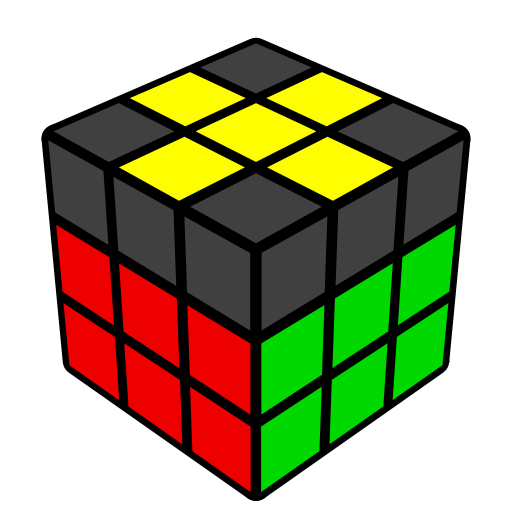
\includegraphics[width=\textwidth]{fakecross.png}
		\caption{Incomplete cross}\label{fig:fakecross}
	\end{subfigure}
	\begin{subfigure}[b]{0.3\textwidth}
		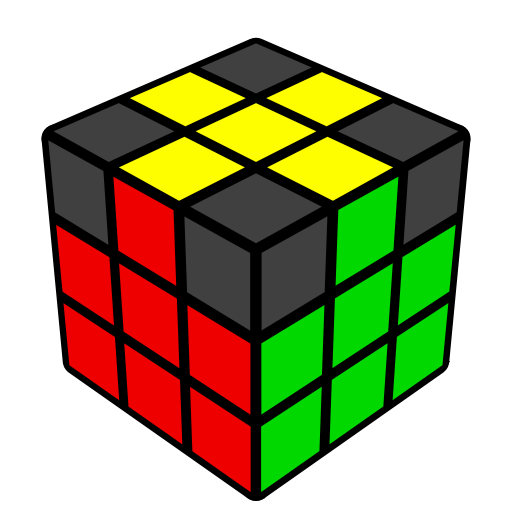
\includegraphics[width=\textwidth]{realcross.png}
		\caption{`Fixed' cross}\label{fig:realcross}
	\end{subfigure}
	\caption{Bottom cross}
\end{figure}

\begin{enumerate}
	\item Flip the white face back to the bottom.
	\item Repeat \alg{FRUR'U'F'} until a cross appears on the yellow face.
	\item Twist the yellow face to fix the cross.
	\item If only two yellow edges can be fixed, there are two cases:\begin{enumerate}
		\item The fixed edges are opposite. In this case, hold the cube such that any one of the fixed yellow edges is in front of you, then do \alg{RUR'URU2R'}. This puts you in the next case.
		\item The fixed edges are adjacent. In this case, do \alg{RUR'URU2R'}. This fixes all edges to complete the stage.
	\end{enumerate}
	\item Flip the white face back up and ensure that none of the previous moves have been disturbed.
\end{enumerate}